Gemeinhin gilt der \textsc{AIDS Information Trojaner} als erste Ransomware im heutigen Sinne, da dieser nicht nur den Computer des Opfers unbrauchbar machte, sondern
		parallel dazu eine "`Reparatur"' gegen Bezahlung anbot. \\
		Getarnt als Anwendung zur Abschätzung des Risikos einer HIV-Infektion und als aktuelle Informationsdatenbank nutzte der 1989 entstandene Virus die damalige
		Unsicherheiten bezüglich einer HIV-Infektion aus, um so eine Installation und auch eine größere Verbreitung zu erreichen.
	\begin{figure}[h!]
		\centering
		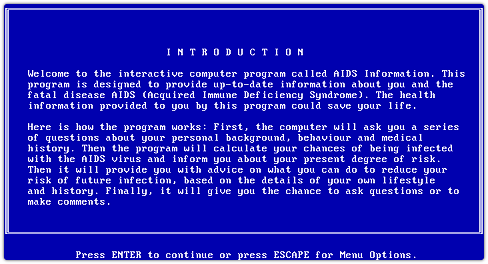
\includegraphics[width=\linewidth]{img/aids1.png}
		\caption{Lizenzvereinbarung AIDS\cite{aids:sophos}}
		\label{fig:lizenz_aids}
	\end{figure}

		Nach der Installation wurde mittels eines Zählers in der Autostart-Datei des Systems ermittelt, wie oft der Computer gestartet worden ist. War der 90. Start
		erreicht, verschlüsselte der Virus die Namen von vordefinierten Dateien und Verzeichnissen, nicht aber deren Inhalt. Dies betraf auch wichtige Systemprogramme, die
		ein Kommando-orientiertes Betriebssystem wie MS-DOS erst benutzbar machen. \\
		Zeitgleich wurde dem Opfer eine Nachricht gezeigt, mit den genauen Anweisungen, wie die vorgebliche Nutzungsgebühr an den Hersteller zu bezahlen sei.
		Scheinbar legitimiert wird dieses Vorgehen mit den Lizenzvereinbarungen, die während der Installation vom Benutzer akzeptiert wurden.

		Eine Analyse des Virus zeigte, dass vor allem die Verwendung einer symmetrischen Verschlüsselung (siehe Kapitel~\ref{sec:sym_verschl}).
		Da hierfür die Schlüssel für die Ver- und Entschlüsselung gleich sind und prinzipbedingt im Virus selbst hinterlegt sein müssen, bot sich hier ein Angriffspunkt, um die
		Verschlüsselung auch ohne Zahlung der geforderten Geldsumme umzukehren. Erleichternd kommt hier dazu, dass die Schlüssel hart-codiert sind, und alle Infektionen
		den gleichen Schlüssel verwenden. \\
		So ist es nicht verwunderlich, dass sich bald Entschlüsselungswerkzeuge verbreiteten und damit die Wirkung des Virus außer Kraft setzten. \\
		Eine Untersuchung durch Adam Young und Moti Yung, schlug hier die Verwendung von asymmetrischer Verschlüsselung (siehe Kapitel ~\ref{sec:asym_verschl}) vor, um einen
		Vorteil über das Opfer zu erhalten. \cite{aids:young}

		Die Autoren heutiger Ransomware haben sich diesen Vorschlag zu Herzen genommen, sodass eine asymmetrische Verschlüsselung heute fast ausnahmslos in Ransomware
		verwendet wird. Auch entscheidende Konzepte von AIDSinfo werden immer noch benutzt, sei des einen vorgeblichen Nutzen des Programms anzubieten oder auch nicht
		direkt nach der Infektion aktiv zu werden, sondern noch einige Zeit abzuwarten.